% Root scan snapshot, with Q1P7 completed by the separate 16 September rescan.
% Scores are feasibility times gain; the original campaign record is unchanged.
\definecolor{scanHigh}{RGB}{21,102,121}
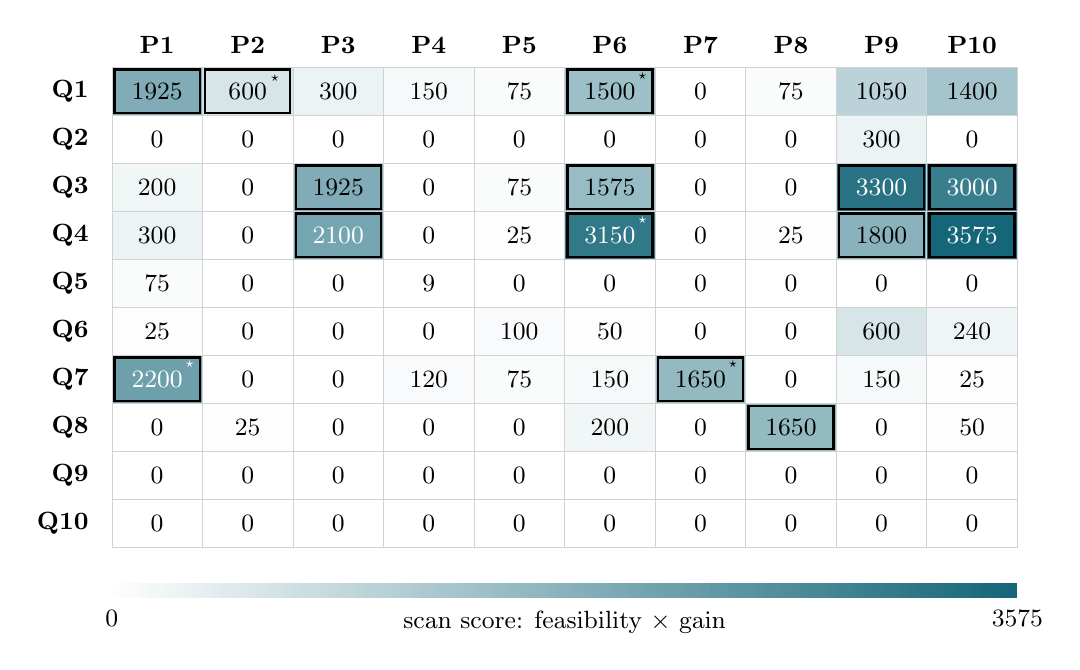
\begin{tikzpicture}[x=1.15cm,y=0.61cm, font=\small]
\node[font=\small\bfseries] at (0.50,0.45) {P1};
\node[font=\small\bfseries] at (1.50,0.45) {P2};
\node[font=\small\bfseries] at (2.50,0.45) {P3};
\node[font=\small\bfseries] at (3.50,0.45) {P4};
\node[font=\small\bfseries] at (4.50,0.45) {P5};
\node[font=\small\bfseries] at (5.50,0.45) {P6};
\node[font=\small\bfseries] at (6.50,0.45) {P7};
\node[font=\small\bfseries] at (7.50,0.45) {P8};
\node[font=\small\bfseries] at (8.50,0.45) {P9};
\node[font=\small\bfseries] at (9.50,0.45) {P10};
\node[anchor=east,font=\small\bfseries] at (-0.15,-0.50) {Q1};
\path[fill=scanHigh!54!white,draw=gray!35,line width=0.25pt] (0,-1) rectangle (1,0);
\node[text=black] at (0.50,-0.50) {1925};
\draw[black,line width=0.85pt] (0.03,-0.95) rectangle (0.97,-0.05);
\path[fill=scanHigh!17!white,draw=gray!35,line width=0.25pt] (1,-1) rectangle (2,0);
\node[text=black] at (1.50,-0.50) {600};
\draw[black,line width=0.85pt] (1.03,-0.95) rectangle (1.97,-0.05);
\node[text=black,font=\tiny,inner sep=0pt] at (1.80,-0.23) {$\star$};
\path[fill=scanHigh!8!white,draw=gray!35,line width=0.25pt] (2,-1) rectangle (3,0);
\node[text=black] at (2.50,-0.50) {300};
\path[fill=scanHigh!4!white,draw=gray!35,line width=0.25pt] (3,-1) rectangle (4,0);
\node[text=black] at (3.50,-0.50) {150};
\path[fill=scanHigh!2!white,draw=gray!35,line width=0.25pt] (4,-1) rectangle (5,0);
\node[text=black] at (4.50,-0.50) {75};
\path[fill=scanHigh!42!white,draw=gray!35,line width=0.25pt] (5,-1) rectangle (6,0);
\node[text=black] at (5.50,-0.50) {1500};
\draw[black,line width=0.85pt] (5.03,-0.95) rectangle (5.97,-0.05);
\node[text=black,font=\tiny,inner sep=0pt] at (5.86,-0.19) {$\star$};
\path[fill=scanHigh!0!white,draw=gray!35,line width=0.25pt] (6,-1) rectangle (7,0);
\node[text=black] at (6.50,-0.50) {0};
\path[fill=scanHigh!2!white,draw=gray!35,line width=0.25pt] (7,-1) rectangle (8,0);
\node[text=black] at (7.50,-0.50) {75};
\path[fill=scanHigh!29!white,draw=gray!35,line width=0.25pt] (8,-1) rectangle (9,0);
\node[text=black] at (8.50,-0.50) {1050};
\path[fill=scanHigh!39!white,draw=gray!35,line width=0.25pt] (9,-1) rectangle (10,0);
\node[text=black] at (9.50,-0.50) {1400};
\node[anchor=east,font=\small\bfseries] at (-0.15,-1.50) {Q2};
\path[fill=scanHigh!0!white,draw=gray!35,line width=0.25pt] (0,-2) rectangle (1,-1);
\node[text=black] at (0.50,-1.50) {0};
\path[fill=scanHigh!0!white,draw=gray!35,line width=0.25pt] (1,-2) rectangle (2,-1);
\node[text=black] at (1.50,-1.50) {0};
\path[fill=scanHigh!0!white,draw=gray!35,line width=0.25pt] (2,-2) rectangle (3,-1);
\node[text=black] at (2.50,-1.50) {0};
\path[fill=scanHigh!0!white,draw=gray!35,line width=0.25pt] (3,-2) rectangle (4,-1);
\node[text=black] at (3.50,-1.50) {0};
\path[fill=scanHigh!0!white,draw=gray!35,line width=0.25pt] (4,-2) rectangle (5,-1);
\node[text=black] at (4.50,-1.50) {0};
\path[fill=scanHigh!0!white,draw=gray!35,line width=0.25pt] (5,-2) rectangle (6,-1);
\node[text=black] at (5.50,-1.50) {0};
\path[fill=scanHigh!0!white,draw=gray!35,line width=0.25pt] (6,-2) rectangle (7,-1);
\node[text=black] at (6.50,-1.50) {0};
\path[fill=scanHigh!0!white,draw=gray!35,line width=0.25pt] (7,-2) rectangle (8,-1);
\node[text=black] at (7.50,-1.50) {0};
\path[fill=scanHigh!8!white,draw=gray!35,line width=0.25pt] (8,-2) rectangle (9,-1);
\node[text=black] at (8.50,-1.50) {300};
\path[fill=scanHigh!0!white,draw=gray!35,line width=0.25pt] (9,-2) rectangle (10,-1);
\node[text=black] at (9.50,-1.50) {0};
\node[anchor=east,font=\small\bfseries] at (-0.15,-2.50) {Q3};
\path[fill=scanHigh!6!white,draw=gray!35,line width=0.25pt] (0,-3) rectangle (1,-2);
\node[text=black] at (0.50,-2.50) {200};
\path[fill=scanHigh!0!white,draw=gray!35,line width=0.25pt] (1,-3) rectangle (2,-2);
\node[text=black] at (1.50,-2.50) {0};
\path[fill=scanHigh!54!white,draw=gray!35,line width=0.25pt] (2,-3) rectangle (3,-2);
\node[text=black] at (2.50,-2.50) {1925};
\draw[black,line width=0.85pt] (2.03,-2.95) rectangle (2.97,-2.05);
\path[fill=scanHigh!0!white,draw=gray!35,line width=0.25pt] (3,-3) rectangle (4,-2);
\node[text=black] at (3.50,-2.50) {0};
\path[fill=scanHigh!2!white,draw=gray!35,line width=0.25pt] (4,-3) rectangle (5,-2);
\node[text=black] at (4.50,-2.50) {75};
\path[fill=scanHigh!44!white,draw=gray!35,line width=0.25pt] (5,-3) rectangle (6,-2);
\node[text=black] at (5.50,-2.50) {1575};
\draw[black,line width=0.85pt] (5.03,-2.95) rectangle (5.97,-2.05);
\path[fill=scanHigh!0!white,draw=gray!35,line width=0.25pt] (6,-3) rectangle (7,-2);
\node[text=black] at (6.50,-2.50) {0};
\path[fill=scanHigh!0!white,draw=gray!35,line width=0.25pt] (7,-3) rectangle (8,-2);
\node[text=black] at (7.50,-2.50) {0};
\path[fill=scanHigh!92!white,draw=gray!35,line width=0.25pt] (8,-3) rectangle (9,-2);
\node[text=white] at (8.50,-2.50) {3300};
\draw[black,line width=0.85pt] (8.03,-2.95) rectangle (8.97,-2.05);
\path[fill=scanHigh!84!white,draw=gray!35,line width=0.25pt] (9,-3) rectangle (10,-2);
\node[text=white] at (9.50,-2.50) {3000};
\draw[black,line width=0.85pt] (9.03,-2.95) rectangle (9.97,-2.05);
\node[anchor=east,font=\small\bfseries] at (-0.15,-3.50) {Q4};
\path[fill=scanHigh!8!white,draw=gray!35,line width=0.25pt] (0,-4) rectangle (1,-3);
\node[text=black] at (0.50,-3.50) {300};
\path[fill=scanHigh!0!white,draw=gray!35,line width=0.25pt] (1,-4) rectangle (2,-3);
\node[text=black] at (1.50,-3.50) {0};
\path[fill=scanHigh!59!white,draw=gray!35,line width=0.25pt] (2,-4) rectangle (3,-3);
\node[text=white] at (2.50,-3.50) {2100};
\draw[black,line width=0.85pt] (2.03,-3.95) rectangle (2.97,-3.05);
\path[fill=scanHigh!0!white,draw=gray!35,line width=0.25pt] (3,-4) rectangle (4,-3);
\node[text=black] at (3.50,-3.50) {0};
\path[fill=scanHigh!1!white,draw=gray!35,line width=0.25pt] (4,-4) rectangle (5,-3);
\node[text=black] at (4.50,-3.50) {25};
\path[fill=scanHigh!88!white,draw=gray!35,line width=0.25pt] (5,-4) rectangle (6,-3);
\node[text=white] at (5.50,-3.50) {3150};
\draw[black,line width=0.85pt] (5.03,-3.95) rectangle (5.97,-3.05);
\node[text=white,font=\tiny,inner sep=0pt] at (5.86,-3.19) {$\star$};
\path[fill=scanHigh!0!white,draw=gray!35,line width=0.25pt] (6,-4) rectangle (7,-3);
\node[text=black] at (6.50,-3.50) {0};
\path[fill=scanHigh!1!white,draw=gray!35,line width=0.25pt] (7,-4) rectangle (8,-3);
\node[text=black] at (7.50,-3.50) {25};
\path[fill=scanHigh!50!white,draw=gray!35,line width=0.25pt] (8,-4) rectangle (9,-3);
\node[text=black] at (8.50,-3.50) {1800};
\draw[black,line width=0.85pt] (8.03,-3.95) rectangle (8.97,-3.05);
\path[fill=scanHigh!100!white,draw=gray!35,line width=0.25pt] (9,-4) rectangle (10,-3);
\node[text=white] at (9.50,-3.50) {3575};
\draw[black,line width=0.85pt] (9.03,-3.95) rectangle (9.97,-3.05);
\node[anchor=east,font=\small\bfseries] at (-0.15,-4.50) {Q5};
\path[fill=scanHigh!2!white,draw=gray!35,line width=0.25pt] (0,-5) rectangle (1,-4);
\node[text=black] at (0.50,-4.50) {75};
\path[fill=scanHigh!0!white,draw=gray!35,line width=0.25pt] (1,-5) rectangle (2,-4);
\node[text=black] at (1.50,-4.50) {0};
\path[fill=scanHigh!0!white,draw=gray!35,line width=0.25pt] (2,-5) rectangle (3,-4);
\node[text=black] at (2.50,-4.50) {0};
\path[fill=scanHigh!0!white,draw=gray!35,line width=0.25pt] (3,-5) rectangle (4,-4);
\node[text=black] at (3.50,-4.50) {9};
\path[fill=scanHigh!0!white,draw=gray!35,line width=0.25pt] (4,-5) rectangle (5,-4);
\node[text=black] at (4.50,-4.50) {0};
\path[fill=scanHigh!0!white,draw=gray!35,line width=0.25pt] (5,-5) rectangle (6,-4);
\node[text=black] at (5.50,-4.50) {0};
\path[fill=scanHigh!0!white,draw=gray!35,line width=0.25pt] (6,-5) rectangle (7,-4);
\node[text=black] at (6.50,-4.50) {0};
\path[fill=scanHigh!0!white,draw=gray!35,line width=0.25pt] (7,-5) rectangle (8,-4);
\node[text=black] at (7.50,-4.50) {0};
\path[fill=scanHigh!0!white,draw=gray!35,line width=0.25pt] (8,-5) rectangle (9,-4);
\node[text=black] at (8.50,-4.50) {0};
\path[fill=scanHigh!0!white,draw=gray!35,line width=0.25pt] (9,-5) rectangle (10,-4);
\node[text=black] at (9.50,-4.50) {0};
\node[anchor=east,font=\small\bfseries] at (-0.15,-5.50) {Q6};
\path[fill=scanHigh!1!white,draw=gray!35,line width=0.25pt] (0,-6) rectangle (1,-5);
\node[text=black] at (0.50,-5.50) {25};
\path[fill=scanHigh!0!white,draw=gray!35,line width=0.25pt] (1,-6) rectangle (2,-5);
\node[text=black] at (1.50,-5.50) {0};
\path[fill=scanHigh!0!white,draw=gray!35,line width=0.25pt] (2,-6) rectangle (3,-5);
\node[text=black] at (2.50,-5.50) {0};
\path[fill=scanHigh!0!white,draw=gray!35,line width=0.25pt] (3,-6) rectangle (4,-5);
\node[text=black] at (3.50,-5.50) {0};
\path[fill=scanHigh!3!white,draw=gray!35,line width=0.25pt] (4,-6) rectangle (5,-5);
\node[text=black] at (4.50,-5.50) {100};
\path[fill=scanHigh!1!white,draw=gray!35,line width=0.25pt] (5,-6) rectangle (6,-5);
\node[text=black] at (5.50,-5.50) {50};
\path[fill=scanHigh!0!white,draw=gray!35,line width=0.25pt] (6,-6) rectangle (7,-5);
\node[text=black] at (6.50,-5.50) {0};
\path[fill=scanHigh!0!white,draw=gray!35,line width=0.25pt] (7,-6) rectangle (8,-5);
\node[text=black] at (7.50,-5.50) {0};
\path[fill=scanHigh!17!white,draw=gray!35,line width=0.25pt] (8,-6) rectangle (9,-5);
\node[text=black] at (8.50,-5.50) {600};
\path[fill=scanHigh!7!white,draw=gray!35,line width=0.25pt] (9,-6) rectangle (10,-5);
\node[text=black] at (9.50,-5.50) {240};
\node[anchor=east,font=\small\bfseries] at (-0.15,-6.50) {Q7};
\path[fill=scanHigh!62!white,draw=gray!35,line width=0.25pt] (0,-7) rectangle (1,-6);
\node[text=white] at (0.50,-6.50) {2200};
\draw[black,line width=0.85pt] (0.03,-6.95) rectangle (0.97,-6.05);
\node[text=white,font=\tiny,inner sep=0pt] at (0.86,-6.19) {$\star$};
\path[fill=scanHigh!0!white,draw=gray!35,line width=0.25pt] (1,-7) rectangle (2,-6);
\node[text=black] at (1.50,-6.50) {0};
\path[fill=scanHigh!0!white,draw=gray!35,line width=0.25pt] (2,-7) rectangle (3,-6);
\node[text=black] at (2.50,-6.50) {0};
\path[fill=scanHigh!3!white,draw=gray!35,line width=0.25pt] (3,-7) rectangle (4,-6);
\node[text=black] at (3.50,-6.50) {120};
\path[fill=scanHigh!2!white,draw=gray!35,line width=0.25pt] (4,-7) rectangle (5,-6);
\node[text=black] at (4.50,-6.50) {75};
\path[fill=scanHigh!4!white,draw=gray!35,line width=0.25pt] (5,-7) rectangle (6,-6);
\node[text=black] at (5.50,-6.50) {150};
\path[fill=scanHigh!46!white,draw=gray!35,line width=0.25pt] (6,-7) rectangle (7,-6);
\node[text=black] at (6.50,-6.50) {1650};
\draw[black,line width=0.85pt] (6.03,-6.95) rectangle (6.97,-6.05);
\node[text=black,font=\tiny,inner sep=0pt] at (6.86,-6.19) {$\star$};
\path[fill=scanHigh!0!white,draw=gray!35,line width=0.25pt] (7,-7) rectangle (8,-6);
\node[text=black] at (7.50,-6.50) {0};
\path[fill=scanHigh!4!white,draw=gray!35,line width=0.25pt] (8,-7) rectangle (9,-6);
\node[text=black] at (8.50,-6.50) {150};
\path[fill=scanHigh!1!white,draw=gray!35,line width=0.25pt] (9,-7) rectangle (10,-6);
\node[text=black] at (9.50,-6.50) {25};
\node[anchor=east,font=\small\bfseries] at (-0.15,-7.50) {Q8};
\path[fill=scanHigh!0!white,draw=gray!35,line width=0.25pt] (0,-8) rectangle (1,-7);
\node[text=black] at (0.50,-7.50) {0};
\path[fill=scanHigh!1!white,draw=gray!35,line width=0.25pt] (1,-8) rectangle (2,-7);
\node[text=black] at (1.50,-7.50) {25};
\path[fill=scanHigh!0!white,draw=gray!35,line width=0.25pt] (2,-8) rectangle (3,-7);
\node[text=black] at (2.50,-7.50) {0};
\path[fill=scanHigh!0!white,draw=gray!35,line width=0.25pt] (3,-8) rectangle (4,-7);
\node[text=black] at (3.50,-7.50) {0};
\path[fill=scanHigh!0!white,draw=gray!35,line width=0.25pt] (4,-8) rectangle (5,-7);
\node[text=black] at (4.50,-7.50) {0};
\path[fill=scanHigh!6!white,draw=gray!35,line width=0.25pt] (5,-8) rectangle (6,-7);
\node[text=black] at (5.50,-7.50) {200};
\path[fill=scanHigh!0!white,draw=gray!35,line width=0.25pt] (6,-8) rectangle (7,-7);
\node[text=black] at (6.50,-7.50) {0};
\path[fill=scanHigh!46!white,draw=gray!35,line width=0.25pt] (7,-8) rectangle (8,-7);
\node[text=black] at (7.50,-7.50) {1650};
\draw[black,line width=0.85pt] (7.03,-7.95) rectangle (7.97,-7.05);
\path[fill=scanHigh!0!white,draw=gray!35,line width=0.25pt] (8,-8) rectangle (9,-7);
\node[text=black] at (8.50,-7.50) {0};
\path[fill=scanHigh!1!white,draw=gray!35,line width=0.25pt] (9,-8) rectangle (10,-7);
\node[text=black] at (9.50,-7.50) {50};
\node[anchor=east,font=\small\bfseries] at (-0.15,-8.50) {Q9};
\path[fill=scanHigh!0!white,draw=gray!35,line width=0.25pt] (0,-9) rectangle (1,-8);
\node[text=black] at (0.50,-8.50) {0};
\path[fill=scanHigh!0!white,draw=gray!35,line width=0.25pt] (1,-9) rectangle (2,-8);
\node[text=black] at (1.50,-8.50) {0};
\path[fill=scanHigh!0!white,draw=gray!35,line width=0.25pt] (2,-9) rectangle (3,-8);
\node[text=black] at (2.50,-8.50) {0};
\path[fill=scanHigh!0!white,draw=gray!35,line width=0.25pt] (3,-9) rectangle (4,-8);
\node[text=black] at (3.50,-8.50) {0};
\path[fill=scanHigh!0!white,draw=gray!35,line width=0.25pt] (4,-9) rectangle (5,-8);
\node[text=black] at (4.50,-8.50) {0};
\path[fill=scanHigh!0!white,draw=gray!35,line width=0.25pt] (5,-9) rectangle (6,-8);
\node[text=black] at (5.50,-8.50) {0};
\path[fill=scanHigh!0!white,draw=gray!35,line width=0.25pt] (6,-9) rectangle (7,-8);
\node[text=black] at (6.50,-8.50) {0};
\path[fill=scanHigh!0!white,draw=gray!35,line width=0.25pt] (7,-9) rectangle (8,-8);
\node[text=black] at (7.50,-8.50) {0};
\path[fill=scanHigh!0!white,draw=gray!35,line width=0.25pt] (8,-9) rectangle (9,-8);
\node[text=black] at (8.50,-8.50) {0};
\path[fill=scanHigh!0!white,draw=gray!35,line width=0.25pt] (9,-9) rectangle (10,-8);
\node[text=black] at (9.50,-8.50) {0};
\node[anchor=east,font=\small\bfseries] at (-0.15,-9.50) {Q10};
\path[fill=scanHigh!0!white,draw=gray!35,line width=0.25pt] (0,-10) rectangle (1,-9);
\node[text=black] at (0.50,-9.50) {0};
\path[fill=scanHigh!0!white,draw=gray!35,line width=0.25pt] (1,-10) rectangle (2,-9);
\node[text=black] at (1.50,-9.50) {0};
\path[fill=scanHigh!0!white,draw=gray!35,line width=0.25pt] (2,-10) rectangle (3,-9);
\node[text=black] at (2.50,-9.50) {0};
\path[fill=scanHigh!0!white,draw=gray!35,line width=0.25pt] (3,-10) rectangle (4,-9);
\node[text=black] at (3.50,-9.50) {0};
\path[fill=scanHigh!0!white,draw=gray!35,line width=0.25pt] (4,-10) rectangle (5,-9);
\node[text=black] at (4.50,-9.50) {0};
\path[fill=scanHigh!0!white,draw=gray!35,line width=0.25pt] (5,-10) rectangle (6,-9);
\node[text=black] at (5.50,-9.50) {0};
\path[fill=scanHigh!0!white,draw=gray!35,line width=0.25pt] (6,-10) rectangle (7,-9);
\node[text=black] at (6.50,-9.50) {0};
\path[fill=scanHigh!0!white,draw=gray!35,line width=0.25pt] (7,-10) rectangle (8,-9);
\node[text=black] at (7.50,-9.50) {0};
\path[fill=scanHigh!0!white,draw=gray!35,line width=0.25pt] (8,-10) rectangle (9,-9);
\node[text=black] at (8.50,-9.50) {0};
\path[fill=scanHigh!0!white,draw=gray!35,line width=0.25pt] (9,-10) rectangle (10,-9);
\node[text=black] at (9.50,-9.50) {0};
\path[fill=scanHigh!1!white,draw=none] (0.00,-11.05) rectangle (0.101,-10.75);
\path[fill=scanHigh!2!white,draw=none] (0.10,-11.05) rectangle (0.201,-10.75);
\path[fill=scanHigh!3!white,draw=none] (0.20,-11.05) rectangle (0.301,-10.75);
\path[fill=scanHigh!4!white,draw=none] (0.30,-11.05) rectangle (0.401,-10.75);
\path[fill=scanHigh!5!white,draw=none] (0.40,-11.05) rectangle (0.501,-10.75);
\path[fill=scanHigh!6!white,draw=none] (0.50,-11.05) rectangle (0.601,-10.75);
\path[fill=scanHigh!7!white,draw=none] (0.60,-11.05) rectangle (0.701,-10.75);
\path[fill=scanHigh!8!white,draw=none] (0.70,-11.05) rectangle (0.801,-10.75);
\path[fill=scanHigh!9!white,draw=none] (0.80,-11.05) rectangle (0.901,-10.75);
\path[fill=scanHigh!10!white,draw=none] (0.90,-11.05) rectangle (1.001,-10.75);
\path[fill=scanHigh!11!white,draw=none] (1.00,-11.05) rectangle (1.101,-10.75);
\path[fill=scanHigh!12!white,draw=none] (1.10,-11.05) rectangle (1.201,-10.75);
\path[fill=scanHigh!13!white,draw=none] (1.20,-11.05) rectangle (1.301,-10.75);
\path[fill=scanHigh!14!white,draw=none] (1.30,-11.05) rectangle (1.401,-10.75);
\path[fill=scanHigh!15!white,draw=none] (1.40,-11.05) rectangle (1.501,-10.75);
\path[fill=scanHigh!16!white,draw=none] (1.50,-11.05) rectangle (1.601,-10.75);
\path[fill=scanHigh!17!white,draw=none] (1.60,-11.05) rectangle (1.701,-10.75);
\path[fill=scanHigh!18!white,draw=none] (1.70,-11.05) rectangle (1.801,-10.75);
\path[fill=scanHigh!19!white,draw=none] (1.80,-11.05) rectangle (1.901,-10.75);
\path[fill=scanHigh!20!white,draw=none] (1.90,-11.05) rectangle (2.001,-10.75);
\path[fill=scanHigh!21!white,draw=none] (2.00,-11.05) rectangle (2.101,-10.75);
\path[fill=scanHigh!22!white,draw=none] (2.10,-11.05) rectangle (2.201,-10.75);
\path[fill=scanHigh!23!white,draw=none] (2.20,-11.05) rectangle (2.301,-10.75);
\path[fill=scanHigh!24!white,draw=none] (2.30,-11.05) rectangle (2.401,-10.75);
\path[fill=scanHigh!25!white,draw=none] (2.40,-11.05) rectangle (2.501,-10.75);
\path[fill=scanHigh!26!white,draw=none] (2.50,-11.05) rectangle (2.601,-10.75);
\path[fill=scanHigh!27!white,draw=none] (2.60,-11.05) rectangle (2.701,-10.75);
\path[fill=scanHigh!28!white,draw=none] (2.70,-11.05) rectangle (2.801,-10.75);
\path[fill=scanHigh!29!white,draw=none] (2.80,-11.05) rectangle (2.901,-10.75);
\path[fill=scanHigh!30!white,draw=none] (2.90,-11.05) rectangle (3.001,-10.75);
\path[fill=scanHigh!31!white,draw=none] (3.00,-11.05) rectangle (3.101,-10.75);
\path[fill=scanHigh!32!white,draw=none] (3.10,-11.05) rectangle (3.201,-10.75);
\path[fill=scanHigh!33!white,draw=none] (3.20,-11.05) rectangle (3.301,-10.75);
\path[fill=scanHigh!34!white,draw=none] (3.30,-11.05) rectangle (3.401,-10.75);
\path[fill=scanHigh!35!white,draw=none] (3.40,-11.05) rectangle (3.501,-10.75);
\path[fill=scanHigh!36!white,draw=none] (3.50,-11.05) rectangle (3.601,-10.75);
\path[fill=scanHigh!37!white,draw=none] (3.60,-11.05) rectangle (3.701,-10.75);
\path[fill=scanHigh!38!white,draw=none] (3.70,-11.05) rectangle (3.801,-10.75);
\path[fill=scanHigh!39!white,draw=none] (3.80,-11.05) rectangle (3.901,-10.75);
\path[fill=scanHigh!40!white,draw=none] (3.90,-11.05) rectangle (4.001,-10.75);
\path[fill=scanHigh!41!white,draw=none] (4.00,-11.05) rectangle (4.101,-10.75);
\path[fill=scanHigh!42!white,draw=none] (4.10,-11.05) rectangle (4.201,-10.75);
\path[fill=scanHigh!43!white,draw=none] (4.20,-11.05) rectangle (4.301,-10.75);
\path[fill=scanHigh!44!white,draw=none] (4.30,-11.05) rectangle (4.401,-10.75);
\path[fill=scanHigh!45!white,draw=none] (4.40,-11.05) rectangle (4.501,-10.75);
\path[fill=scanHigh!46!white,draw=none] (4.50,-11.05) rectangle (4.601,-10.75);
\path[fill=scanHigh!47!white,draw=none] (4.60,-11.05) rectangle (4.701,-10.75);
\path[fill=scanHigh!48!white,draw=none] (4.70,-11.05) rectangle (4.801,-10.75);
\path[fill=scanHigh!49!white,draw=none] (4.80,-11.05) rectangle (4.901,-10.75);
\path[fill=scanHigh!50!white,draw=none] (4.90,-11.05) rectangle (5.001,-10.75);
\path[fill=scanHigh!51!white,draw=none] (5.00,-11.05) rectangle (5.101,-10.75);
\path[fill=scanHigh!52!white,draw=none] (5.10,-11.05) rectangle (5.201,-10.75);
\path[fill=scanHigh!53!white,draw=none] (5.20,-11.05) rectangle (5.301,-10.75);
\path[fill=scanHigh!54!white,draw=none] (5.30,-11.05) rectangle (5.401,-10.75);
\path[fill=scanHigh!55!white,draw=none] (5.40,-11.05) rectangle (5.501,-10.75);
\path[fill=scanHigh!56!white,draw=none] (5.50,-11.05) rectangle (5.601,-10.75);
\path[fill=scanHigh!57!white,draw=none] (5.60,-11.05) rectangle (5.701,-10.75);
\path[fill=scanHigh!58!white,draw=none] (5.70,-11.05) rectangle (5.801,-10.75);
\path[fill=scanHigh!59!white,draw=none] (5.80,-11.05) rectangle (5.901,-10.75);
\path[fill=scanHigh!60!white,draw=none] (5.90,-11.05) rectangle (6.001,-10.75);
\path[fill=scanHigh!61!white,draw=none] (6.00,-11.05) rectangle (6.101,-10.75);
\path[fill=scanHigh!62!white,draw=none] (6.10,-11.05) rectangle (6.201,-10.75);
\path[fill=scanHigh!63!white,draw=none] (6.20,-11.05) rectangle (6.301,-10.75);
\path[fill=scanHigh!64!white,draw=none] (6.30,-11.05) rectangle (6.401,-10.75);
\path[fill=scanHigh!65!white,draw=none] (6.40,-11.05) rectangle (6.501,-10.75);
\path[fill=scanHigh!66!white,draw=none] (6.50,-11.05) rectangle (6.601,-10.75);
\path[fill=scanHigh!67!white,draw=none] (6.60,-11.05) rectangle (6.701,-10.75);
\path[fill=scanHigh!68!white,draw=none] (6.70,-11.05) rectangle (6.801,-10.75);
\path[fill=scanHigh!69!white,draw=none] (6.80,-11.05) rectangle (6.901,-10.75);
\path[fill=scanHigh!70!white,draw=none] (6.90,-11.05) rectangle (7.001,-10.75);
\path[fill=scanHigh!71!white,draw=none] (7.00,-11.05) rectangle (7.101,-10.75);
\path[fill=scanHigh!72!white,draw=none] (7.10,-11.05) rectangle (7.201,-10.75);
\path[fill=scanHigh!73!white,draw=none] (7.20,-11.05) rectangle (7.301,-10.75);
\path[fill=scanHigh!74!white,draw=none] (7.30,-11.05) rectangle (7.401,-10.75);
\path[fill=scanHigh!75!white,draw=none] (7.40,-11.05) rectangle (7.501,-10.75);
\path[fill=scanHigh!76!white,draw=none] (7.50,-11.05) rectangle (7.601,-10.75);
\path[fill=scanHigh!77!white,draw=none] (7.60,-11.05) rectangle (7.701,-10.75);
\path[fill=scanHigh!78!white,draw=none] (7.70,-11.05) rectangle (7.801,-10.75);
\path[fill=scanHigh!79!white,draw=none] (7.80,-11.05) rectangle (7.901,-10.75);
\path[fill=scanHigh!80!white,draw=none] (7.90,-11.05) rectangle (8.001,-10.75);
\path[fill=scanHigh!81!white,draw=none] (8.00,-11.05) rectangle (8.101,-10.75);
\path[fill=scanHigh!82!white,draw=none] (8.10,-11.05) rectangle (8.201,-10.75);
\path[fill=scanHigh!83!white,draw=none] (8.20,-11.05) rectangle (8.301,-10.75);
\path[fill=scanHigh!84!white,draw=none] (8.30,-11.05) rectangle (8.401,-10.75);
\path[fill=scanHigh!85!white,draw=none] (8.40,-11.05) rectangle (8.501,-10.75);
\path[fill=scanHigh!86!white,draw=none] (8.50,-11.05) rectangle (8.601,-10.75);
\path[fill=scanHigh!87!white,draw=none] (8.60,-11.05) rectangle (8.701,-10.75);
\path[fill=scanHigh!88!white,draw=none] (8.70,-11.05) rectangle (8.801,-10.75);
\path[fill=scanHigh!89!white,draw=none] (8.80,-11.05) rectangle (8.901,-10.75);
\path[fill=scanHigh!90!white,draw=none] (8.90,-11.05) rectangle (9.001,-10.75);
\path[fill=scanHigh!91!white,draw=none] (9.00,-11.05) rectangle (9.101,-10.75);
\path[fill=scanHigh!92!white,draw=none] (9.10,-11.05) rectangle (9.201,-10.75);
\path[fill=scanHigh!93!white,draw=none] (9.20,-11.05) rectangle (9.301,-10.75);
\path[fill=scanHigh!94!white,draw=none] (9.30,-11.05) rectangle (9.401,-10.75);
\path[fill=scanHigh!95!white,draw=none] (9.40,-11.05) rectangle (9.501,-10.75);
\path[fill=scanHigh!96!white,draw=none] (9.50,-11.05) rectangle (9.601,-10.75);
\path[fill=scanHigh!97!white,draw=none] (9.60,-11.05) rectangle (9.701,-10.75);
\path[fill=scanHigh!98!white,draw=none] (9.70,-11.05) rectangle (9.801,-10.75);
\path[fill=scanHigh!99!white,draw=none] (9.80,-11.05) rectangle (9.901,-10.75);
\path[fill=scanHigh!100!white,draw=none] (9.90,-11.05) rectangle (10.001,-10.75);
\node[anchor=north] at (0,-11.12) {0};
\node[anchor=north] at (10,-11.12) {3575};
\node[anchor=north] at (5,-11.12) {scan score: feasibility $\times$ gain};
\end{tikzpicture}
